\thispagestyle{duongvaotoanhocnone}
\pagestyle{duongvaotoanhoc}
\everymath{\color{duongvaotoanhoc}}
\graphicspath{{../duongvaotoanhoc/pic/}}
\blfootnote{$^1$\color{duongvaotoanhoc}Viện Toán học.}
\begingroup
\AddToShipoutPicture*{\put(0,616){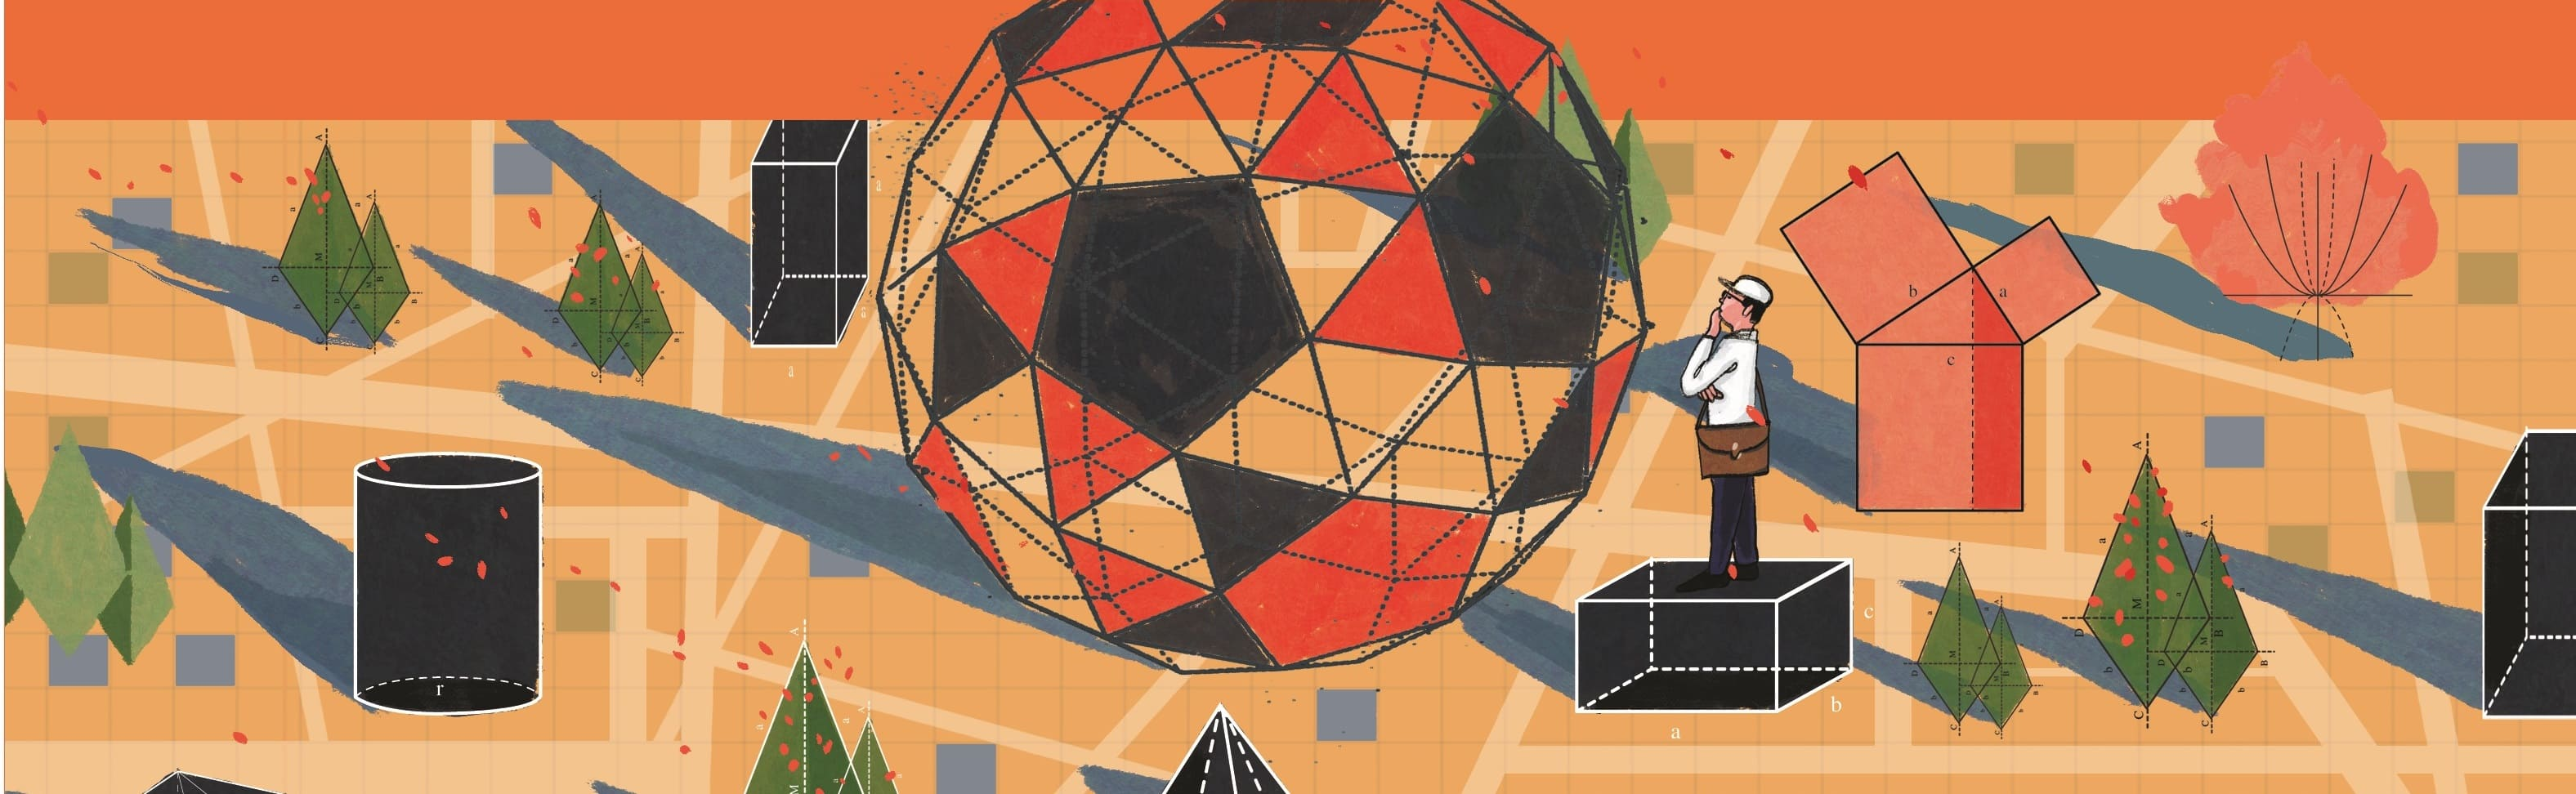
\includegraphics[width=19.3cm]{../bannerduongvao}}}
\AddToShipoutPicture*{\put(168,553){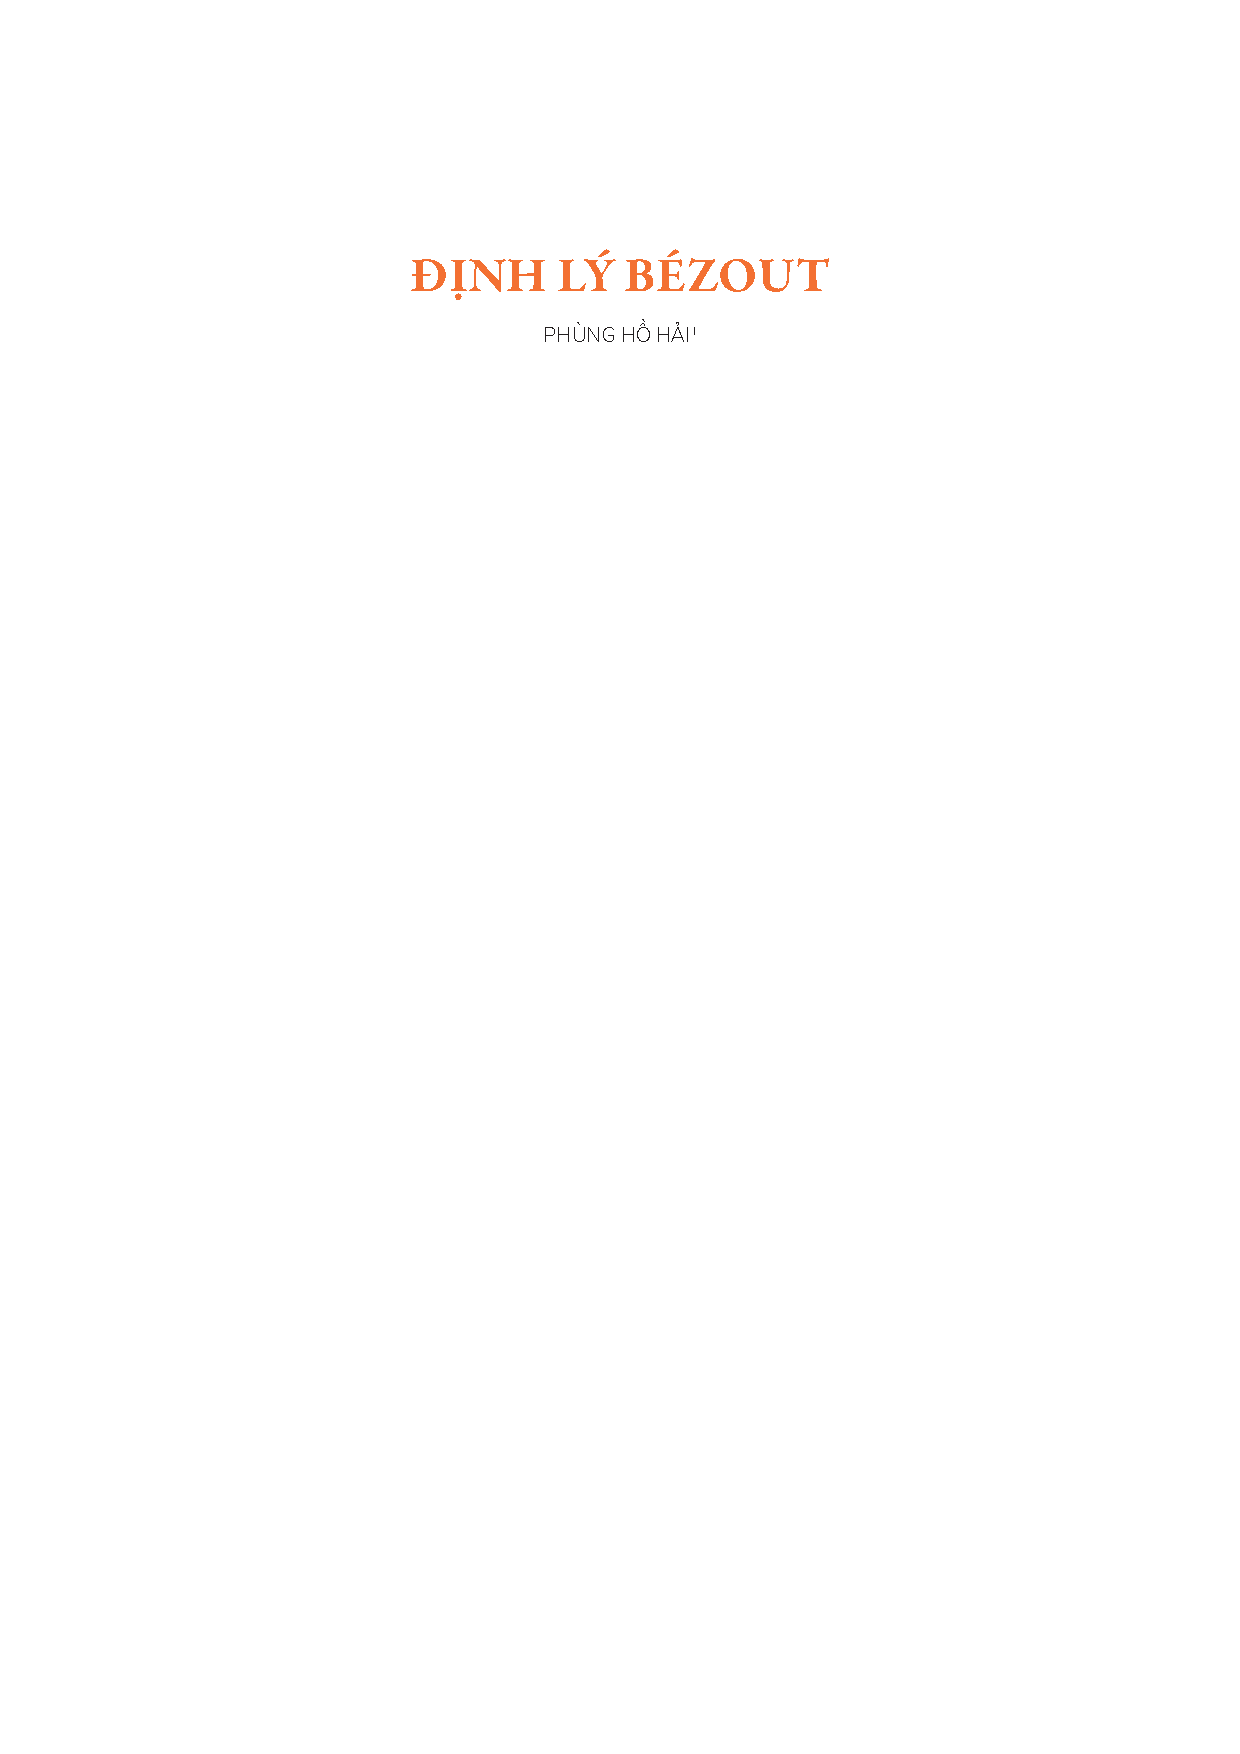
\includegraphics[scale=1]{../tieude.pdf}}}
\centering
\endgroup
\vspace*{154pt}

\begin{multicols}{2}	
	Chúng ta biết rằng một đa thức hệ bậc $n\geq 1$ với hệ số thực có không quá $n$ nghiệm thực. Điều này cũng có thể được minh họa là đồ thị của nó cắt trục hoành tại không quá $n$ điểm. Tổng quát hơn ta có: đồ thi  đó cắt một đường thẳng bất kỳ cũng tại không quá $n$ điểm. 
	\begin{figure}[H]
		\centering
		\vspace*{-5pt}
		\captionsetup{labelformat= empty, justification=centering}
		\begin{tikzpicture}[scale=0.52, duongvaotoanhoc, node font= \small]
			\begin{axis} [axis lines=center]
				\addplot [blue,domain=-2.5:2.5, smooth] { x^3 - 4*x };
				\addplot [domain=-5:5,red,smooth] {2};
				\addplot [domain=-5:5,green,smooth] {4};
			\end{axis}
		\end{tikzpicture}
		\caption{\small\textit{\color{duongvaotoanhoc}Hình $1$.}}
		\vspace*{-10pt}
	\end{figure}
	Nếu cho hai đường elipse trên mặt phẳng cắt nhau ta thấy số giao điểm không thể quá $4$. Điều này cũng đúng với các đường parabola và hyperbola.
	\vskip 0.1cm
	Nếu cho một elipse cắt đồ thị của một đa thức bậc $3$ thì số giao điểm có thể lên tới $6$. Ta thấy, số giao điểm lớn nhất có thể liên quan tới bậc của các đường cong mà ta đang xét.
	\begin{figure}[H]
		\centering
		\vspace*{-5pt}
		\captionsetup{labelformat= empty, justification=centering}
		\begin{tikzpicture}[duongvaotoanhoc,scale=0.52, node font= \small]
			\begin{axis}[domain=-5:5, axis x line=bottom,axis y line=left]
				\addplot [blue,domain=-2.5:2.5, smooth] { x^3 - 4*x };
			\end{axis}
			\draw[red] (3.5,3) ellipse (3.3cm and 1cm);
		\end{tikzpicture}
		\caption{\small\textit{\color{duongvaotoanhoc}Hình $2$.}}
		\vspace*{-5pt}
	\end{figure}
	Nếu xét đa thức hệ số phức và các nghiệm phức, đồng thời tính cả bội thì một đa thức bậc $n\geq 1$ với hệ số phức có đúng $n$ nghiệm. Ta cũng có thể nói, ``đồ thị'' của đa thức này cắt ``đường thẳng phức'' tại đúng $n$ điểm nếu tính cả bội.
	\vskip 0.1cm
	Định lý Bézout phát biểu rằng {\em hai đường cong đại số trên mặt phẳng xạ ảnh cắt nhau tại đúng $n$ điểm nếu kể cả bội, với $n$ là tích của bậc của hai đường cong} (ngoại trừ trường hợp chúng trùng nhau một phần). 
	\vskip 0.1cm
	Khẳng định về số giao điểm của hai đường cong trên mặt phẳng đã được phát biểu nhiều lần trong nhiều tác phẩm bởi các nhà toán học nổi tiếng như Newton ($1665$), Maclaurin ($1720$), Euler và Cramber ($1748$). Tuy nhiên trước Etienne Bézout ($1730-1783$), chưa có một chứng minh cụ thể nào được đưa ra. 
	\vskip 0.1cm
	Bézout đưa ra chứng minh năm $1779$ trong cuốn sách {\em Théorie générale des équations algébraiques} (Lý thuyết đại cương về phương trình đại số). Một đường cong đại số trên mặt phẳng được xác định như tập nghiệm của một đa thức hai biến. Như vậy khẳng định có thể được phát biểu như là số nghiệm của một hệ hai phương trình đa thức theo hai ẩn.
	Bézout đã đưa ra khái niệm {\em kết thức} để giải quyết bài toán. Cho hai đa thức $F(x)$ và $G(x)$ hệ số phức với bậc tương ứng là $m$ và $n$. Ký hiệu $\mathbb C[x]_d$ là không gian véc tơ các đa thức với bậc nhỏ hơn $d$. Xét ánh xạ tuyến tính ``Bézout'' cho bởi 
	\setlength{\abovedisplayskip}{5pt}
	\setlength{\belowdisplayskip}{5pt}
	\begin{align*}
		\mathbb C[x]_n\!\times\! \mathbb C[x]_m \!\rightarrow\!  \mathbb C[x]_{m\!+\!n},
		(A,B)\!\mapsto\! AF\!+\!BG.
	\end{align*}
	Nhận xét là số chiều của hai không gian nguồn và đích cùng bằng $m+n$. Do đó ta có thể xét định thức của ánh xạ này. Đây chính là kết thức của $F$ và $G$. Theo bổ đề Bézout (xem Bổ đề $2$ dưới đây), nếu $F$ và $G$ có nghiệm chung thì ánh xạ trên có hạch không tầm thường, từ đó kết thức bằng $0$, và ngược lại. 
	\vskip 0.1cm
	Bằng cách coi hai đa thức theo $x$ và $y$ như là các đa thức theo biến $y$, thì kết thức của chúng sẽ là một đa thức theo $x$ với bậc không vượt quá tích các bậc của hai đa thức ban đầu. Từ đó Bézout có một chứng minh cho các đa thức (và do đó các đường cong) ở vị trí tổng quát. 
	\vskip 0.1cm
	Một chứng minh chặt chẽ và bao quát hết mọi khả năng chỉ được đưa ra bởi Georges--Henri Halphen năm $1873$. 
	Khó khăn trong việc phát biểu và chứng minh dạng tổng quát của định lý Bézout là việc định nghĩa khái niệm bội của giao điểm của hai đường cong đại số. J.--P. Serre ($1965$) đề xuất giải quyết vấn đề này một cách triệt để thông qua vành địa phương. Đây cũng có thể coi là một trong những điểm xuất phát của Hình học Đại số hiện đại. 
	\vskip 0.1cm
	$\pmb{1.}$ \textbf{\color{duongvaotoanhoc}Đường cong cho bởi phương trình đa thức}
	\vskip 0.1cm
	Một đường thẳng trong mặt phẳng được xác định bởi phương trình  
	\begin{align*}
		ax+by+c=0
	\end{align*}
	trong đó ít nhất một trong hai số $a$ hoặc $b$ khác $0$. Tương tự, một đường cong bậc $2$, còn gọi là đường conic, được xác định bởi phương trình
	\begin{align*}
		ax^2+bxy+cx^2+dx+ey+g=0,
	\end{align*}
	với ít nhất một trong các hệ số $a,b,c$ khác $0$.
	\vskip 0.1cm
	Tổng quát, một {\em đường cong đại số} trên mặt phẳng (còn gọi tắt là đường cong phẳng) được định nghĩa như là tập nghiệm của một đa thức hai biến (khác hằng số):
	\begin{align*}
		F(x,y)=0. \tag{$1$}
	\end{align*}
	Ở đây $F$ là một đa thức theo hai biến $x$ và $y$:
	\begin{align*}
		F(x,y)=\sum_{i,j} a_{ij}x^iy^j,
	\end{align*}
	trong đó tổng ở vế phải là một tổng hữu hạn. Tổng lớn nhất các số mũ trong các đơn thức $x^iy^j$ ở vế phải được gọi là {\em bậc} của $F$, ký hiệu $\deg F$. 
	\vskip 0.1cm
	Xét {\em họ các đường cong} xác định bởi phương trình
	\begin{align*}
		(ax+by+c)^2-\alpha=0,
	\end{align*}
	với $\alpha$ thay đổi. Khi $\alpha\neq 0$ phương trình này xác định một cặp hai đường thẳng song song. Khi $\alpha$ tiến tới $0$, hai đường thẳng này tiến gần tới nhau và khi $\alpha=0$, hai đường thẳng này tạo thành {\em một đường thẳng kép}. 
	\vskip 0.1cm
	Như vậy hình ảnh hình học của tập nghiệm không phản ánh hết bản chất đại số của phương trình, đặc biệt khi phương trình đó phụ thuộc vào tham số. Để giải quyết vấn đề này, ta sẽ sử dụng {\em ngôn ngữ đại số} để mô tả hình học. Định nghĩa của một đường cong đại số vì thế sẽ được phát biểu như sau. 
	\vskip 0.2cm
	\PIbox{\em Đường cong đại số trong mặt phẳng được xác định bởi một đa thức $F\in \mathbb C[x,y]$ có bậc lớn hơn hoặc bằng 1, tập các điểm hình học của nó là nghiệm của phương trình $F$. Đường cong đại số này được gọi tắt là {\em đường cong $F$}. }
	\vskip 0.2cm
	Trong Hình học Đại số, thay vì xét các tập nghiệm thực của phương trình ($1$), người ta xét các nghiệm phức. Có một số khác biệt căn bản giữa nghiệm thực và nghiệm phức, từ góc độ đại số cũng như từ góc độ hình học. 
	\vskip 0.1cm
	($1$) Một trong những tính chất đại số quan trọng nhất của số phức là mọi đa thức hệ số phức với bậc $n\geq 1$ đều có đủ $n$ nghiệm phức, nếu tính cả bội.   
	\vskip 0.1cm 
	($2$) Từ góc độ hình học chúng ta biết rằng tập các số phức lập thành một mặt phẳng, thường gọi là {\em mặt phẳng phức}. Do đó tập các số phức có chiều hình học bằng $2$. Như vậy, một đường cong phức cũng có số chiều bằng $2$. 
	\vskip 0.1cm
	($3$) Để phân biệt mặt phẳng phức với không gian tuyến tính phức hai chiều ta sẽ gọi không gian này là {\em mặt phẳng affine phức}. Chữ ``affine'' hàm ý ta chỉ xét nó như một không gian tuyến tính và chỉ quan tâm tới các tính chất song song hay cắt nhau của các đường thẳng, hoặc tính thẳng hàng hay không thẳng hàng của các điểm, mà không quan tâm tới các yếu tố như góc hay khoảng cách. 
	\vskip 0.1cm
	($4$) Việc hình dung hình học các đường cong đại số phức tương đối khó. Ví dụ hai đường thẳng phức trong không gian phức hai chiều thường cắt nhau tại duy nhất một điểm. Nhìn từ góc độ hình học điều đó có nghĩa là hai mặt phẳng trong không gian bốn chiều cắt nhau tại một điểm. 
	\vskip 0.1cm
	($5$) Do đó, để thuận tiện cho tư duy hình học, đôi khi ta sử dụng ``phần thực'' của một đường cong phức, khi nó được xác định như là tập nghiệm của một đa thức hệ số thực. Tuy nhiên chúng ta cần cảnh giác rằng nhiều kết luận đúng đối với phần thực, có thể không đúng đối với toàn bộ đường cong phức. 
	\vskip 0.1cm
	Ví dụ xét tập nghiệm của phương trình
	\begin{align*}
		xy-1=0.
	\end{align*}
	Đây là một hyperbola. Phần thực của nó bao gồm hai nhánh rời nhau. 
	Thực hiện một phép đổi biến với hệ số phức:
	$x'=(x+y)/2;\ y'=(x-y)/2i$, ta có
	\begin{align*}
		{x'}^2+{y'}^2=xy=1.
	\end{align*}
	Nghĩa là nếu ``cắt'' đường cong phức $xy-1=0$ bởi mặt phẳng thực căng trên hai véc tơ $x'$ và $y'$ thì ta thu được một đường tròn. 
	\vskip 0.1cm
	Thực tế, toàn bộ đường cong là một mặt hai chiều liên thông! 
	Để thấy rõ hơn điều này ta biểu diễn các biến phức $x$ và $y$ theo các biến thực:
	\begin{align*}
		x=u+iv\text{ và } y=w+iz.
	\end{align*}
	Phương trình trên được đưa về dạng:
	\begin{align*}
		\begin{cases}
			 uw-vz=1\\
			 uz+vw=0.
		\end{cases}
	\end{align*}
	Từ đó ta suy ra
	\begin{align*}
		t:=\frac uw=-\frac vz\neq 0.
	\end{align*}
	Thế vào phương trình đầu ta thu được
	\begin{align*}
		u^2+v^2=t.
	\end{align*}
	\begin{figure}[H]
		\vspace*{-5pt}
		\centering
		\captionsetup{labelformat= empty, justification=centering}
		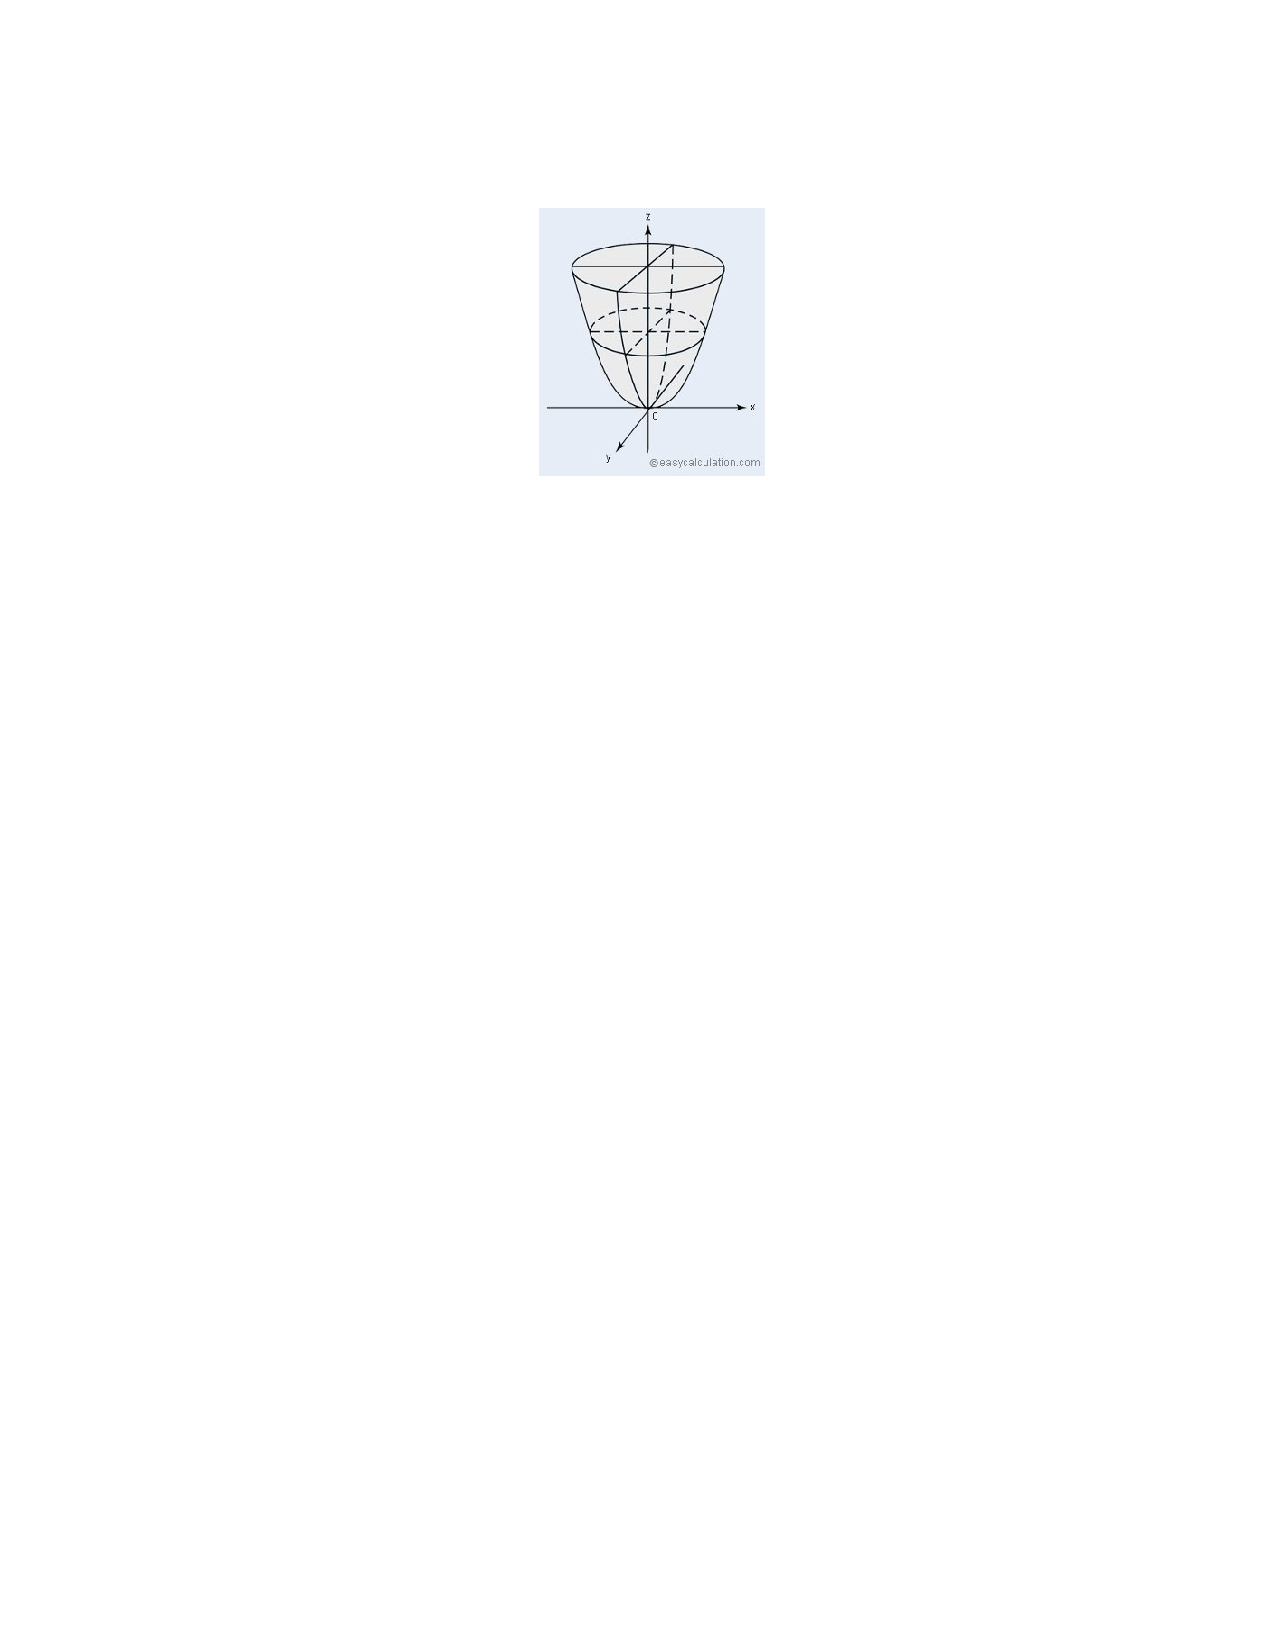
\includegraphics[width= 0.55\linewidth]{3}
		\caption{\small\textit{\color{duongvaotoanhoc}Hình $3$.}}
		\vspace*{-10pt}
	\end{figure}
	Như vậy:
	\vskip 0.2cm
	\PIbox{trong không gian $3$ chiều với các tọa độ là $u,v,t$, nghiệm của phương trình xác định {\bf\color{duongvaotoanhoc} đường hyperbola phức} lập thành một {\bf\color{duongvaotoanhoc} mặt paraboloid tròn xoay thực}, bỏ đi điểm $(0,0,0)$ (ứng với giá trị $t=0$).}
	\vskip 0.2cm
	$\pmb{2.}$ \textbf{\color{duongvaotoanhoc}Đường cong  bất khả quy}
	\vskip 0.1cm 
	Nếu đa thức $F$ phân tích thành hai đa thức $G$ và $H$, bậc $>0$, thì tập nghiệm của $F=$ là hợp các tập nghiệm của $G=0$ và $H=0$. Một đa thức được gọi là {\em bất khả quy} nếu nó không có phân tích như trên. Đường cong xác định bởi đa thức này cũng được gọi là {\em bất khả quy}. Kết quả sau đây khẳng định rằng một đường cong đại số sẽ là hợp của các đường cong bất khả quy.
	\vskip 0.1cm
	\textbf{\color{duongvaotoanhoc}Định lý} $\pmb{1.}$ \textit{Một đa thức hai biến với hệ số phức luôn phân tích được theo một cách duy nhất (sai khác các hệ số khác 0) thành tích các đa thức bất khả quy.}
	\vskip 0.1cm 
	Phân tích đa thức $F$ ra các thành phần bất khả quy:
	\begin{align*}
		F =\prod_{i=1}^r F_i{}^{d_i},\quad d_i\geq 1.
	\end{align*}
	Khi đó đường cong $F$  là hợp của các đường cong $F_i$. Ta cũng nói mỗi đường cong  $F_i$ là một {\em thành phần bất khả quy} của đường cong  $F$. Số $d_i$ được gọi là số bội của thành phần bất khả quy tương ứng. 
	\vskip 0.1cm
	Chứng minh của định lý $1$ là mẫu mực cho cách tiếp cận sơ cấp tới các đa thức nhiều biến. Ý tưởng cơ bản là đưa việc xét đa thức theo hai biến $x,y$ về việc xét các đa thức theo biến $x$ với hệ số là các đa thức theo biến $y$, sau đó ta mở rộng tập các hệ số ra các phân thức đại số theo $y$. Phương pháp này tương tự như khi ta sử dụng các đa thức với hệ số hữu tỷ để giải quyết bài toán cho các đa thức hệ số nguyên. 
	\vskip 0.1cm
	Các bạn học sinh giỏi toán bậc THPT rất nên thử tìm cách chứng minh định lý trên. Ý tưởng chứng minh sử dụng bổ đề quen thuộc của Bézout và  Gauss cho đa thức hai biến. 
	\vskip 0.1cm
	Dưới đây là phát biểu của các bổ đề này cho các đa thức hệ số nguyên. 
	\vskip 0.1cm
	\textbf{\color{duongvaotoanhoc}Bổ đề} $\pmb{2}$ (Bézout)\textbf{\color{duongvaotoanhoc}.} \textit{Cho hai số nguyên $m$ và $n$. Khi đó tồn tại các số nguyên $k$ và $l$ sao cho }
		\begin{align*}
			k\cdot m+l\cdot n=\textrm{\rm UCLN}(m,n).
		\end{align*}
	\vskip 0.1cm
	\textbf{\color{duongvaotoanhoc}Bổ đề} $\pmb{3}$ (Gauss)\textbf{\color{duongvaotoanhoc}.}
	\textit{Đối với một đa thức $P(x)$ với hệ số nguyên ta định nghĩa {\em  dung lượng} của $P(x)$ là ước chung lớn nhất của các hệ số của $P(x)$, ký hiệu là $c(P)$. Đa thức $P(x)$ được gọi là {\em rút gọn} nếu $c(P)=1$. Với hai đa thức hệ số nguyên tùy ý $P(x)$, $Q(x)$ ta luôn có}
	\begin{align*}
		c(P\cdot Q)=c(P)\cdot c(Q).
	\end{align*}
	Vành đa thức $\mathbb C[x]$ có nhiều tính chất số học giống vành các số nguyên. Cụ thể, trong đó cũng có thể thực hiện được phép chia có dư. Tập các phân thức hữu tỷ $\mathbb C(x)$ đóng vai trò tương tự như tập các số hữu tỷ. 
	Việc phát biểu và chứng minh các kết quả tương tự với bổ đề Gauss và Bézout cho các đa thức hai biến dành cho bạn đọc.  
	\vskip 0.1cm	
	$\pmb{3.}$ \textbf{\color{duongvaotoanhoc}Điểm đơn và tiếp tuyến}
	\vskip 0.1cm
	Tiếp tuyến tới đồ thị của đa thức $P(x)$ tại điểm $x=a$, $y=P(a)$ được cho bởi phương trình
	\begin{align*}
		y-P(a)=P'(a)(x-a).
	\end{align*}
	Ta có thể mở rộng kết quả này cho một đường cong đại số bất kỳ cho bởi đa thức $F(x,y)$. Giả sử $P(a,b)$ là một điểm trên đường cong (nghĩa là $F(a,b)=0$). Nếu một trong hai đạo hàm riêng 
	\begin{align*}
		F_x:=\frac{\partial F}{\partial x} \textrm{ hoặc } F_y:=\frac{\partial F}{\partial y}
	\end{align*}
	khác $0$ tại $P$ thì tiếp tuyến tại $P$ tới đường cong được cho bởi phương trình:
	\begin{align*}
		F_x(a,b)(x-a)+F_y(a,b) (y-b)=0. \tag{$2$}
	\end{align*}
	Có nhiều cách để lý giải điều này. Cách đơn giản nhất là thông qua khai triển Taylor đối với $F$ tại điểm $P(a,b)$. Do $F(a,b)=0$ nên khai triển này có dạng:
	\begin{align*}
		F(x,y)=&F_1(x-a,y-b)\\
		&+F_2(x-a,y-b)+\ldots,
	\end{align*}
	trong đó $F_1(x-a,y-b)= F_x(a,b)(x-a)+F_y(a,b)(y-b)$, còn các số hạng $F_2(x-a,y-b)$... có bậc cao hơn theo $x-a$ và $y-b$.  Do tiếp tuyến tới một đường cong tại một điểm $P$ trên đường cong mô tả \textit{xấp xỉ tuyến tính} của phần đường cong tại xung quanh điểm $P$, ta kết luận, phương trình của tiếp tuyến được cho bởi công thức ($2$).
	\vskip 0.1cm
	Nhận xét rằng khai triển Taylor của một đa thức thực ra chính là sắp xếp các đơn thức theo lũy thừa tăng dần, sau khi đã đổi biến đưa điểm đang xét về gốc tọa độ: $(x,y)\mapsto (x-a,y-b)$. 
	\vskip 0.1cm
	\PIbox{Một điểm trên đường cong $F$ được gọi là \textbf{\color{duongvaotoanhoc}điểm đơn} nếu ít nhất một đạo hàm riêng của $F$ tại điểm đó khác $0$.  }
	\vskip 0.1cm
	\textbf{\color{duongvaotoanhoc}Ví dụ.} Khai triển Taylor của đa thức 
	$F(x,y)=x^2+y^2$ 
	tại điểm $A(1,2)$ được cho bởi
	\begin{align*}
		F(x,y)=\,&((x-1)+1)^2+((y-2)+2)^2\\
		=\,&F(1,2)+[2(x-1)+4(y-2)]\\
		&+[(x-1)^2+(y-2)^2].
	\end{align*}
	Do điểm $A(1,2)$ nằm trên đường cong $F-5=0$ nên tiếp tuyến tại đó được cho bởi phương trình
	\begin{align*}
		2(x-1)+4(y-2)=0.
	\end{align*}
	$\pmb{4.}$ \textbf{\color{duongvaotoanhoc}Điểm bội và tiếp tuyến}
	\vskip 0.1cm 
	Một điểm trên đường cong $F$  được gọi là điểm bội nếu nó không phải là điểm đơn. Trước tiên ta sẽ xét trường hợp $F$ là một đa thức bất khả quy trong $\mathbb C[x,y]$. Để đơn giản ta sẽ giả thiết điểm đang xét là gốc tọa độ $O(0,0)$. Các hình vẽ dưới đây mô tả ``phần thực'' của một số đường cong tại lân cận điểm $O$:
	\begin{figure}[H]
		\vspace*{-10pt}
		\centering
		\captionsetup{labelformat= empty, justification=centering}
		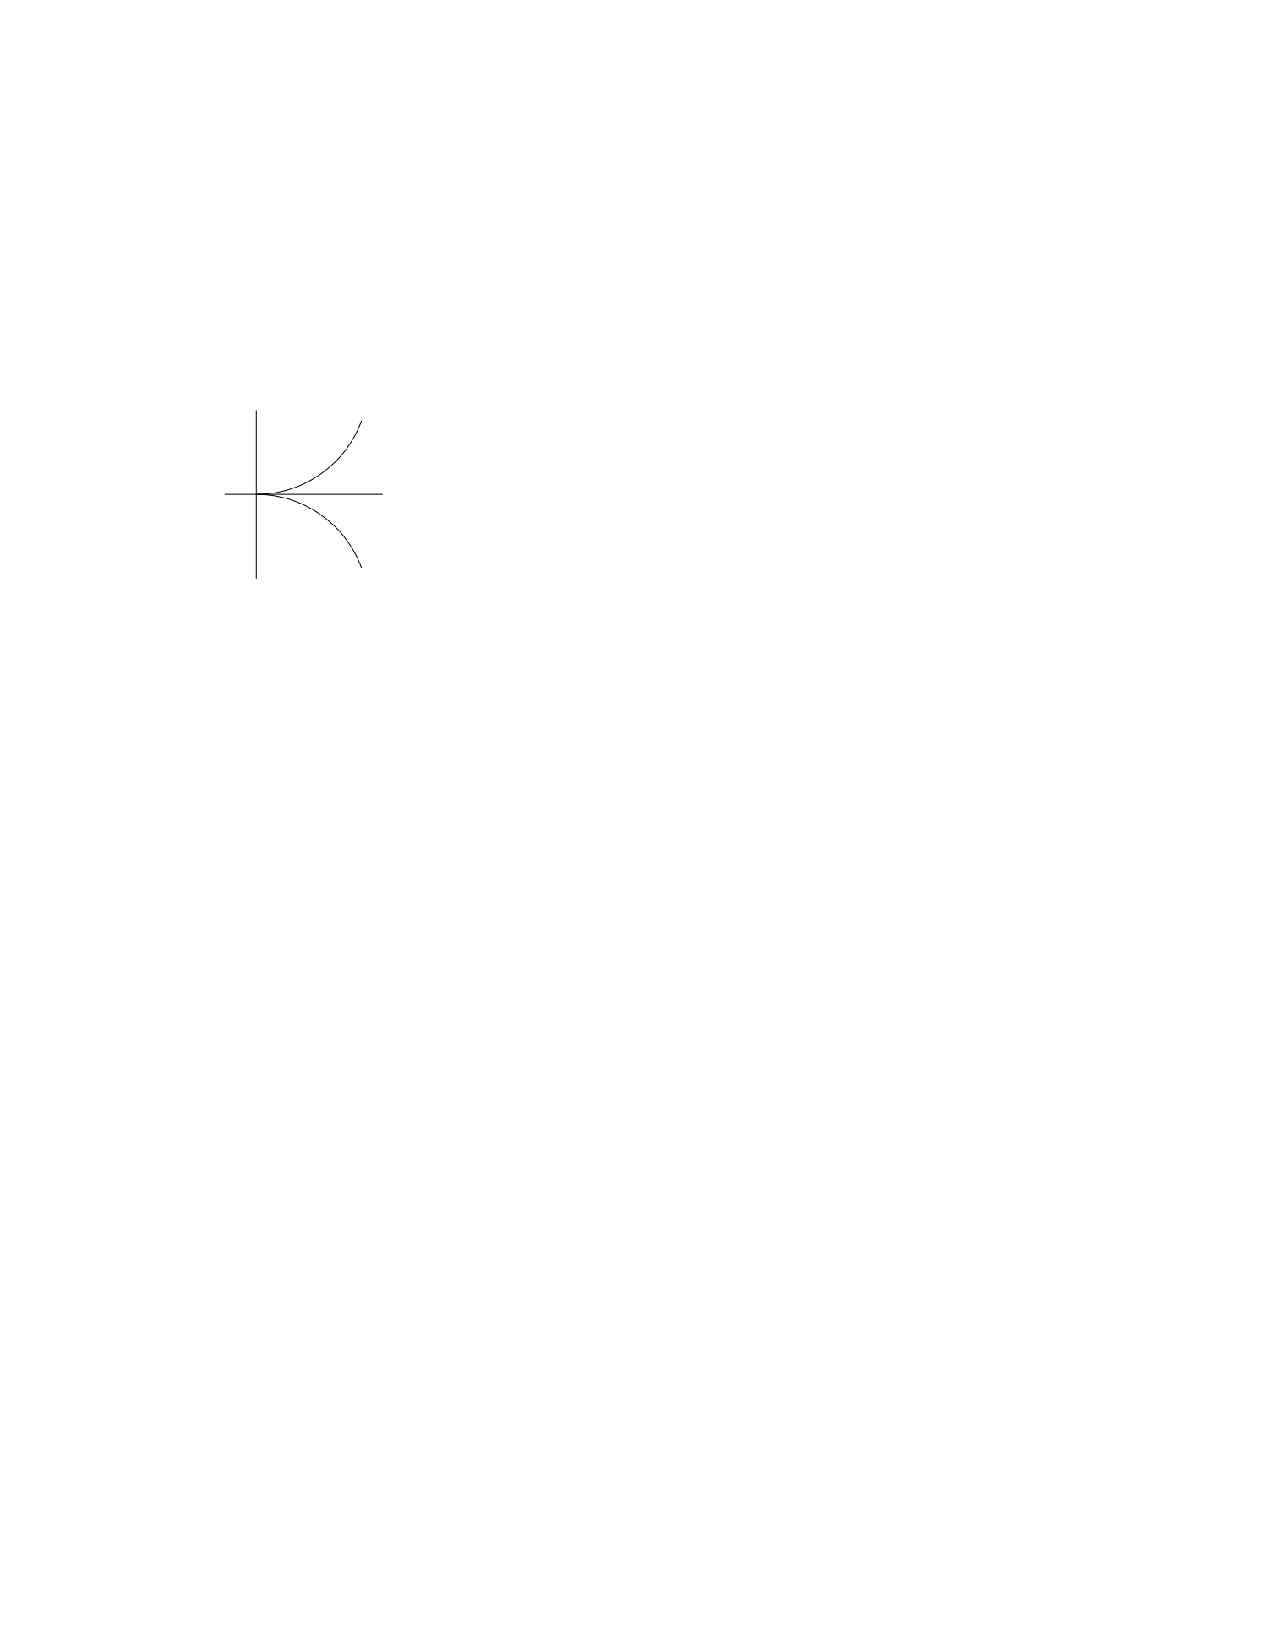
\includegraphics[scale=0.8]{4a}\quad\quad
		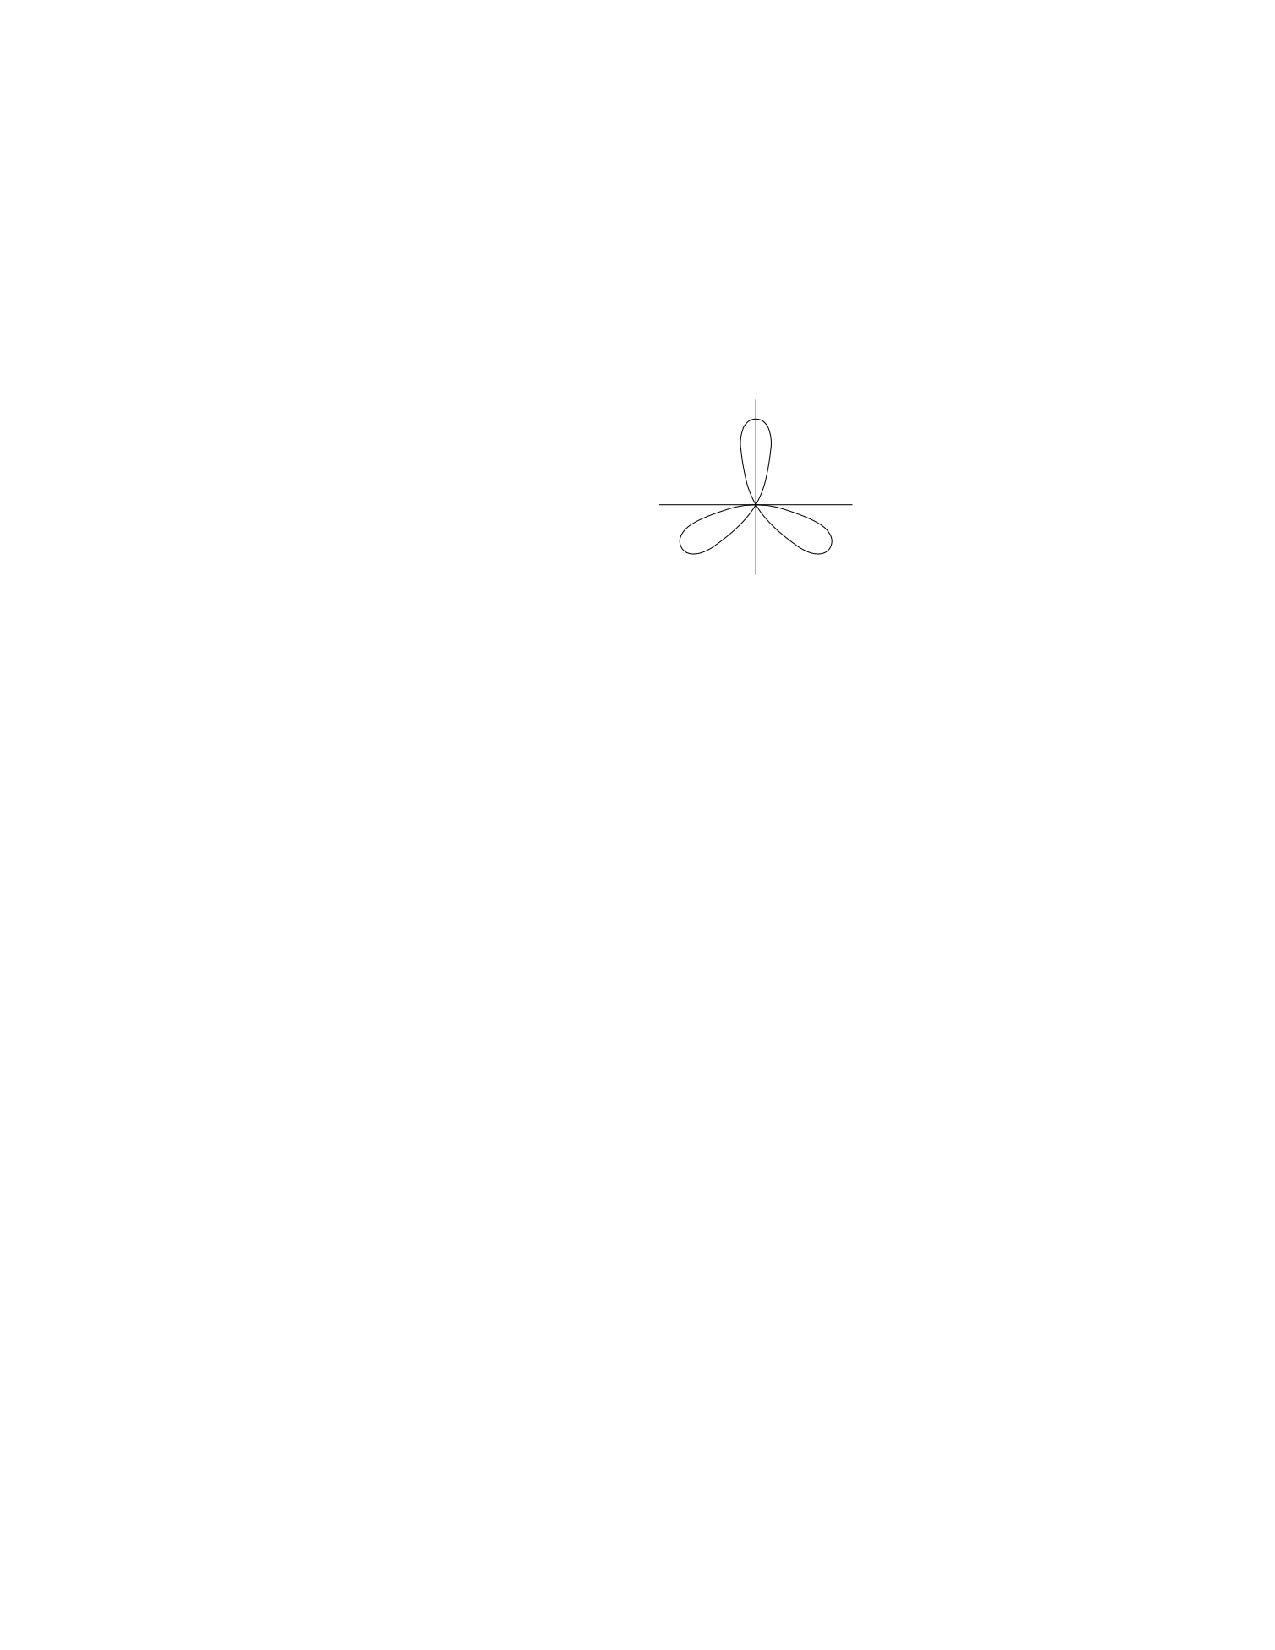
\includegraphics[scale=0.8]{4c}
		\caption{\small$F=x^3-y^2$ \quad\quad\quad$F\!=\!(x^2 \!+\! y^2)^2 \!+\! 3x^2y\!-\!y^3$}
		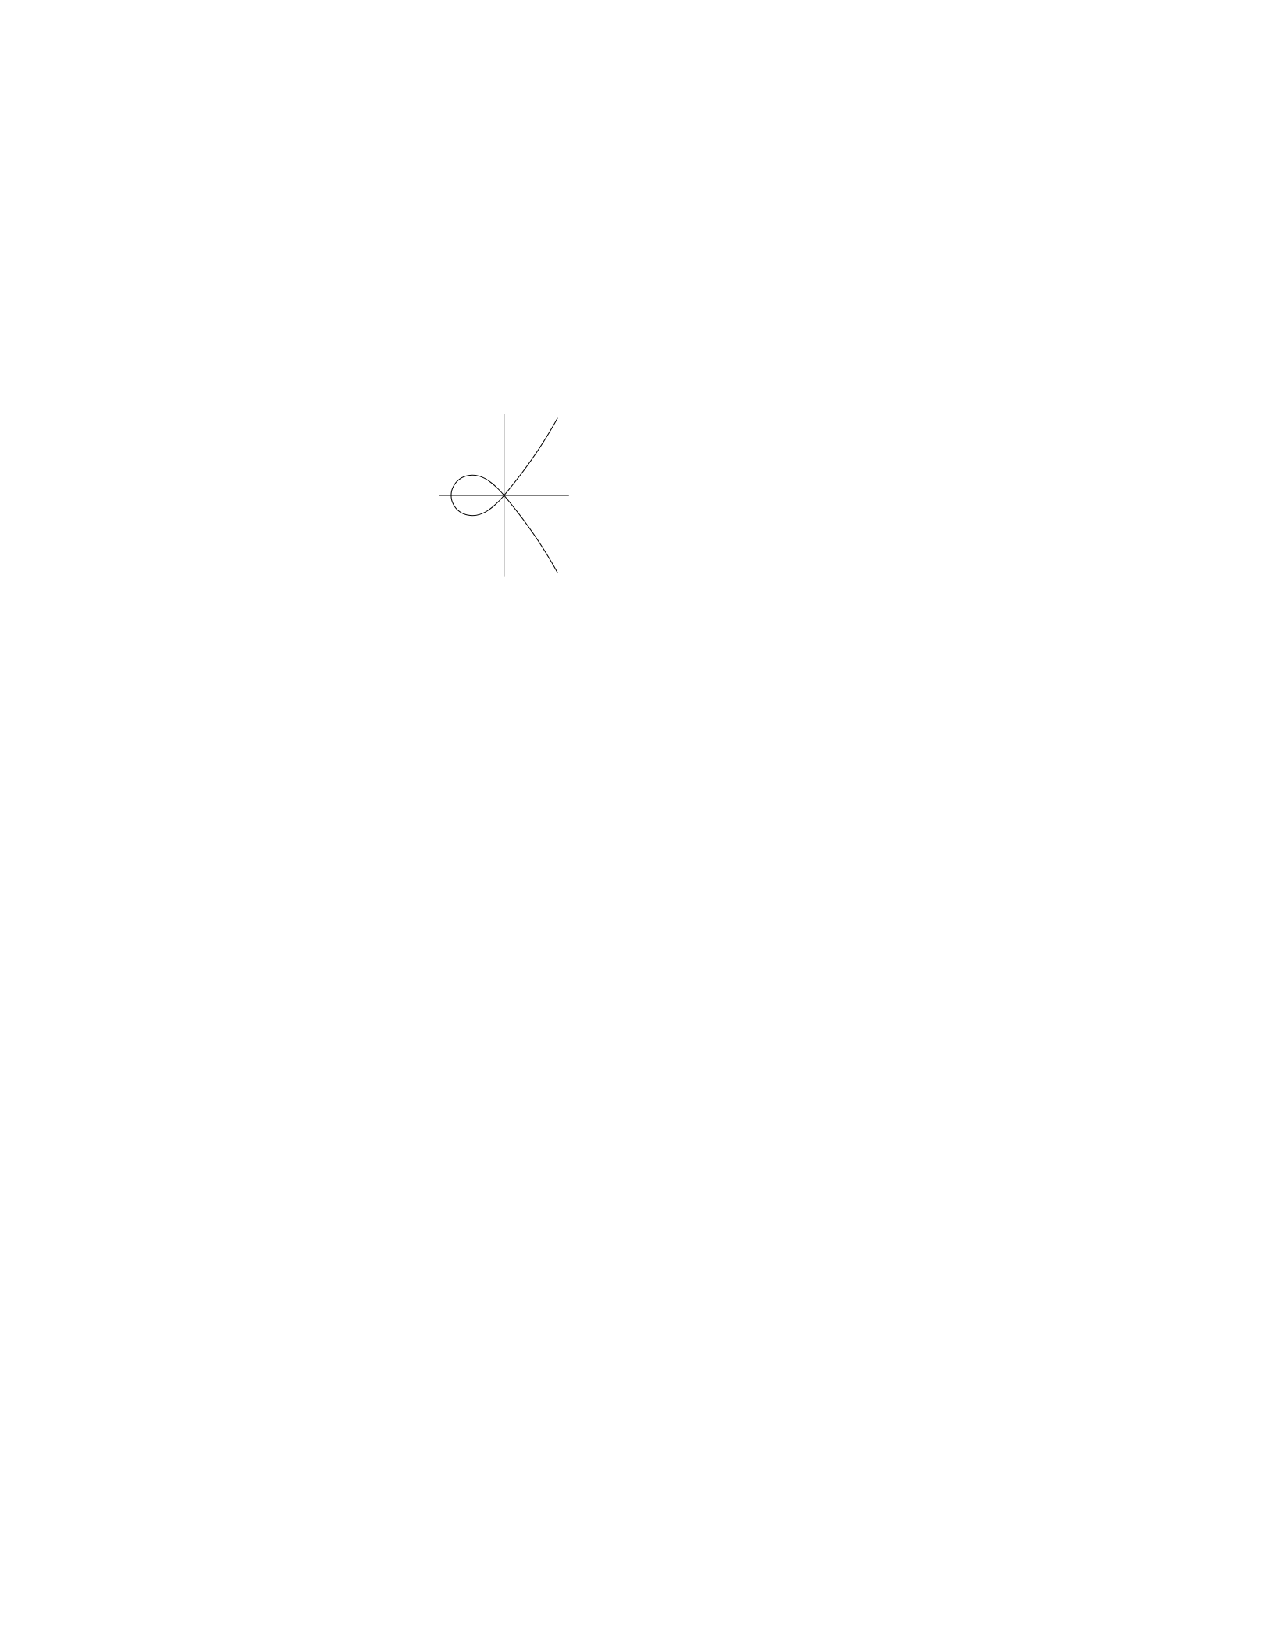
\includegraphics[scale=0.8]{4b}\quad\quad\quad
		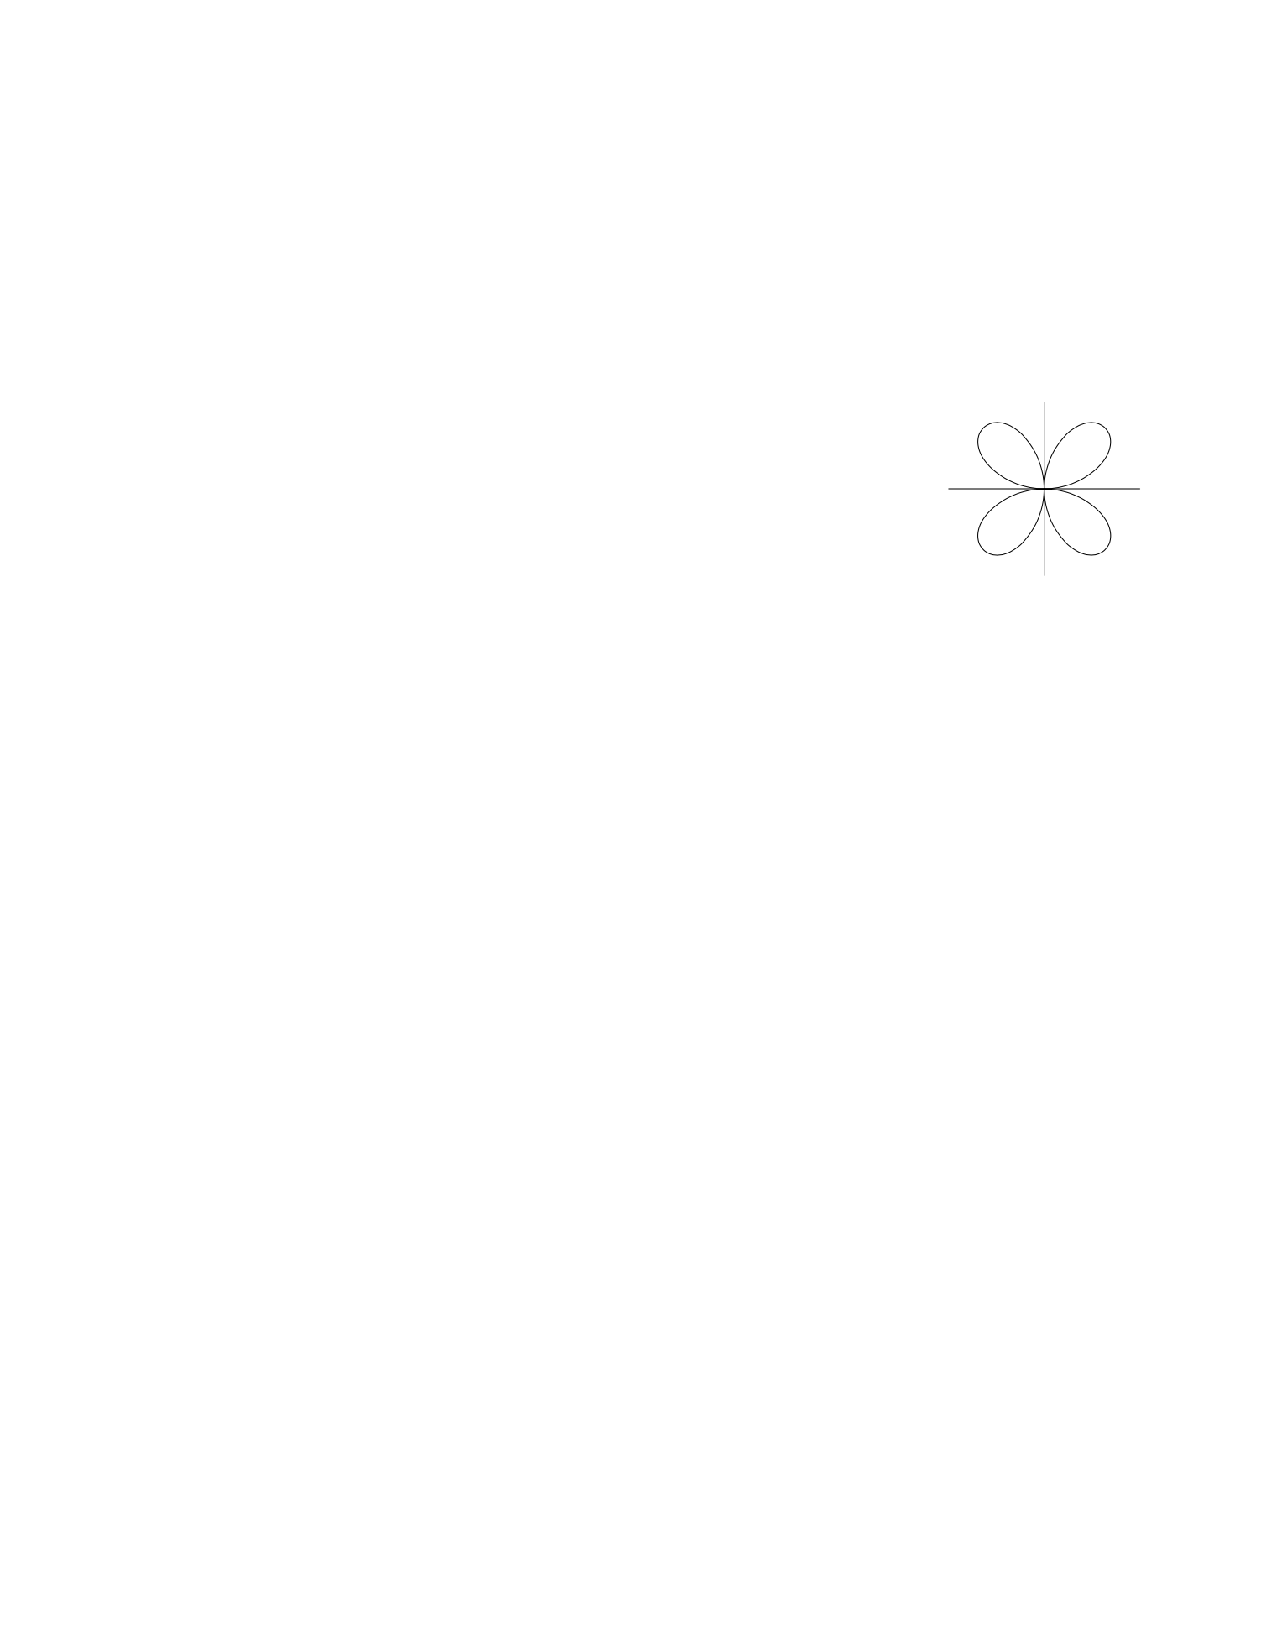
\includegraphics[scale=0.8]{4d}
		\caption{\small$F=x^3+x^2-y^2$ \quad$F=(x^2 + y^2)^3- 4x^2y^2$}
		\caption{\small\textit{\color{duongvaotoanhoc}Hình $4$. Các đường cong với kỳ dị tại $O(0,0)$.}}
		\vspace*{-5pt}
	\end{figure}
	Nhắc lại rằng nếu điểm $O(0,0)$ là điểm bội của $F(x,y)$ khai triển Taylor của $F$ tại $O$ có dạng
	\begin{align*}
		F=F_m+F_{m+1}+\ldots, \quad m\geq 2,
	\end{align*}
	trong đó $F_i$ là các đa thức thuần nhất bậc $i$ theo $x$ và $y$. 
	\vskip 0.1cm
	Trong các đồ thị ở hình $4$, giá trị $m$ tương ứng là $2,2,3,4$. Phương trình
	$F_m=0$
	tương ứng là:
	\begin{align*}
		y^2&=0\\
		x^2-y^2&=0\\
		3x^2y-y^3&=0\\
		4x^2y^2&=0.
	\end{align*} 
	Các phương trình này xác định các chùm đường thẳng (bao gồm cả đường thẳng kép) là các tiếp tuyến tới đường cong tại $O$. 
	\vskip 0.1cm
	Ta thấy giá trị của $m$ ứng với số các tiếp tuyến tới đường cong tại điểm $O$. Lý giải cho điều này rất đơn giản. 
	\vskip 0.2cm
	\PIbox{Trong một {\em lân cận đủ nhỏ} của $O$, $F$ được xấp xỉ bởi $F_m$, do đó đường cong  $F$  được xấp xỉ bởi đường cong $F_m$.}
	\vskip 0.2cm
	Mở rộng phân tích ở trên cho một điểm bất kỳ trên đường cong ta có định nghĩa sau. 
	Cho $F\in \mathbb C[x,y]$ là đa thức bất khả quy và $P(a,b)$ là một điểm trên đường cong $F$. 
	\vskip 0.2cm
	\PIbox{Bội của $P$ trên đường cong, ký hiệu là $\mu_P(F)$, là lũy thừa nhỏ nhất trong khai triển Taylor của $F$ tại $P$:
	\begin{align*}
		F(x,y)= &F_m(x-a,y-b)\\
		&+F_{m+1}(x-a,y-b)+\ldots
	\end{align*}
		Phương trình
		$F_m(x-a,y-b)=0$
		xác định các đường thẳng tiếp xúc với đương cong tại $P$. }
	\vskip 0.2cm
	Nếu hai đường cong $F$  và $G$  cắt nhau tại điểm $P$, thì bội giao tại $P$ của hai đường cong phụ thuộc vào vị trí tương đối của các tiếp tuyến của hai đường cong. Trong trường hợp các tiếp tuyến là đôi một phân biệt thì bội giao sẽ là tích của số các tiếp tuyến. Nhưng trong trường hợp có sự trùng lấp thì vấn đề chưa rõ ràng. 
	\vskip 0.1cm
	Về nguyên tắc, để xác định được bội giao, người ta thực hiện một phép biến dạng nhỏ hai đường cong tại lân cận của giao điểm, sau đó đếm số giao điểm của hai đường cong trong lân cận đó. Đó là phương pháp của Giải tích. Trong Hình học Đại số, ta sẽ sử dụng tiếp cận khác, trong đó ta sẽ trừu tượng hóa vấn đề lên để qua đó nhìn thấy sâu hơn bản chất của nó. Bội giao của hai đường cong sẽ được nhìn nhận như chiều của các không gian véc tơ. Công cụ để triển khai việc này là {\em vành địa phương}. 
	\vskip 0.1cm
	$\pmb{5.}$ \textbf{\color{duongvaotoanhoc}Vành địa phương và bội của điểm trên đường cong} 
	\vskip 0.1cm 
	Thay vì xác định bội của một điểm trên đường cong như là số các giao điểm nào đó, ta có thể xác định số bội này thông qua vành địa phương. Ý tưởng mấu chốt ở đây là vành địa phương tại một điểm trên đường cong {\em chứa toàn bộ thông tin về hình học} của đường cong trong lân cận của điểm đó. Sau khi đã nhìn thấy điều đó thì việc xây dựng các công thức là vấn đề mang tính kỹ thuật. 
	\vskip 0.1cm
	Nhắc lại rằng số bội của một điểm $P$ trên đường cong $F$ được xác định nhờ khai triển Taylor của $F$ tại điểm đó. Ta sẽ định nghĩa số bội này thông qua số chiều của các không gian véc tơ được xây dựng từ vành địa phương của $P$.  Ưu điểm của cách làm này là nó cho một mô tả trừu tượng về số bội, cho chúng ta hiểu biết sâu sắc hơn về nó, để từ đó cho phép phát triển những phương pháp hiện đại hơn khi nghiên cứu số bội. 
	\vskip 0.1cm
	{\em Vành địa phương tại một điểm trong mặt phẳng affine} (phức) được hiểu là tập các hàm số xác định trên một lân cận nào đó của điểm đã cho. Do ta chỉ xét các hàm ``đại số'' nên định nghĩa của một hàm địa phương là như sau.
	\vskip 0.2cm
	\PIbox{Vành địa phương $\pazocal O_P$ tại điểm $P(a,b)$ trong mặt phẳng affine là tập hợp các phân thức đại số $F/G$ với tính chất
		$G(P):=G(a,b)\neq 0.$}
	\vskip 0.2cm
	Tập hợp các phân thức trong $\pazocal O_P$ triệt tiêu tại $P$ lập thành ideal cực đại duy nhất trong vành này, ký hiệu là $\mathfrak m_P$. 
	\begin{align*}
		\mathfrak m_P=\left\{ F/G \left|\right.  F(P)=0, G(P)\neq 0\right\}.
	\end{align*}
	Trong Đại số Giao hoán, một vành với duy nhất ideal cực đại được gọi   là \textbf{\color{duongvaotoanhoc}vành địa phương}.
	\vskip 0.1cm
	Cho $P(a,b)$ là một điểm trên đường cong bất khả quy  $F$. Các hàm địa phương trên mặt phẳng affine tại $P$ khi hạn chế lên đường cong này xác định các hàm địa phương trên đó. Ta nhận thấy rằng hai hàm khi hạn chế lên đường cong sẽ bằng nhau nếu chúng sai khác nhau bởi một bội số của $F$. Do đó, 
	\vskip 0.2cm
	\PIbox{vành các hàm địa phương tại $P$ trên đường cong $F$  là vành thương 
		$\pazocal O_P(F):= \pazocal O_P/(F),$}
	\vskip 0.2cm
	trong đó $(F)$ là ideal sinh bởi $F$ trong vành $\pazocal O_P$.
	Vành $\pazocal O_P(F)$ cũng là vành địa phương với ideal cực đại duy nhất:
	$\mathfrak m_P(F)=\mathfrak m_P/(F).$
	\vskip 0.1cm
	\textbf{\color{duongvaotoanhoc}Mệnh đề} $\pmb{4}$ (Bội của điểm trên đường cong)\textbf{\color{duongvaotoanhoc}.} 
		\textit{Cho $F\in\mathbb C[x,y]$ là đa thức bất khả quy và $P$ là một điểm trên đường cong $F$. 
		Khi đó với mọi $n\geq\mu:= \mu_P(F)$  ta có} 
		\begin{align*}
			\dim_{\mathbb C}  \pazocal O_P(F)/(\mathfrak m_P(F)^n)=\mu \cdot n -
			{\mu \choose 2}.
		\end{align*}
	\vskip 0.1cm
	Trong trường hợp $P$ là một điểm đơn trên đường cong, nghĩa là $\mu_P(F)=1$, từ công thức trên ta suy ra:
	\begin{align*}
		\dim_{\mathbb C} \mathfrak m_P(F)^n/\mathfrak m_P(F)^{n+1}=1
	\end{align*}
	với mọi $n$. 
	\vskip 0.1cm
	\columnbreak
	$\pmb{6.}$ \textbf{\color{duongvaotoanhoc}Giao điểm của hai đường cong}
	\vskip 0.1cm
	Xét hai đường cong $F$  và $G$. Khi đó hệ phương trình
	\begin{align*}
		\begin{cases}
			F = 0\\
			G = 0
		\end{cases}
	\end{align*}
	xác định tập giao của hai đường cong này.  
	\vskip 0.1cm
	\textbf{\color{duongvaotoanhoc}Định lý} $\pmb{5.}$ \textit{Giả thiết hai đường cong $F$  và $G$  không chứa chung một thành phần, khi đó chúng giao nhau tại một tập hữu hạn điểm.}
	\vskip 0.1cm
	\textit{Chứng minh.}
	Theo giả thiết thì hai đa thức $F$ và $G$ không có ước chung trong $\mathbb C[x,y]$. Khi đó hai đa thức này cũng không có ước chung trong $\mathbb C(x)[y]$ -- tập các đa thức theo $y$ với hệ số trong $\mathbb C(x)$. Từ đó, theo bổ để B\'ezout, tồn tại hai đa thức $A$ và $B$ trong  $\mathbb C(x)[y]$ sao cho
	\begin{align*}
		1=AF+BG.
	\end{align*}
	Sau khi quy đồng mẫu số các hệ số của $A$ và $B$ ta thu được đẳng thức
	\begin{align*}
		C= A'F+ B'G,
	\end{align*}
	với $0\neq C\in\mathbb C[x]$, $ A', B'\in \mathbb C[x,y]$. 
	Như vậy nghiệm của hệ $(F=0, G=0)$ có tọa độ theo trục $x$ là nghiệm của đa thức {\em một biến} $C$, do đó là tập hữu hạn. Lý luận tương tự đối với tọa độ $y$ ta suy ra điều phải chứng minh. 
	\vskip 0.1cm
	$\pmb{7.}$ \textbf{\color{duongvaotoanhoc}Xạ ảnh hóa mặt phẳng affine} 
	\vskip 0.1cm
	Trong mặt phẳng affine phức, tồn tại các đường cong không giao nhau tại điểm nào, ví dụ hai đường thẳng song song. 
	Đây có thể được hiểu như một trường hợp {\em suy biến}. Xét hệ sau:
	\begin{align*}
		\begin{cases}
			\alpha x+y+1 =0\\
			y=0
		\end{cases}
	\end{align*}
	Với mọi $\alpha\neq 0$, hệ có duy nhất nghiệm, với $\alpha=0$, hệ vô nghiệm. 
	\vskip 0.1cm
	Ta hình dung khi $\alpha$ {\em tiến tới} $0$, giao điểm của hai đường thẳng $y=0$ và $\alpha x+y+1=0$ {\em chạy ra vô cùng}. Ta sẽ bổ sung {\em điểm ở vô cùng} này vào mặt phẳng affine. Mỗi đường thẳng trên mặt phẳng affine sẽ xác định một điểm ở vô cùng. Hai đường thẳng song song cùng xác định một điểm tại vô cùng là điểm mà chúng cắt nhau. 
	\vskip 0.1cm
	Mặt phẳng affine bổ sung thêm các điểm ở vô cùng được gọi là {\em mặt phẳng xạ ảnh}. Các điểm trong mặt phẳng xạ ảnh (thực hoặc phức) được mô tả thuận tiện nhất thông qua các tọa độ thuần nhất. Một tọa độ thuần nhất là một dãy tỷ lệ $[a_0:a_1:a_2]$ trong đó có ít nhất một trong các tọa độ $a_i\neq 0$. Nhắc lại rằng hai dãy tỷ lệ $[a_0:a_1:a_2]$ và $[b_0:b_1:b_2]$ được gọi là bằng nhau nếu tồn tại $\lambda\neq 0$ sao cho
	\begin{align*}
		a_i=\lambda b_i, \quad i=0,1,2.
	\end{align*}
	Một điểm trong mặt phẳng affine với tọa độ $(a_0,a_1)$ sẽ có tọa độ thuần nhất $[a_0:a_1:1]$. Các điểm ở vô cùng có tọa độ dạng $[a_0:a_1:0]$ (với ít nhất một trong hai số $a_0$, $a_1$ khác $0$). Điểm này ứng với đường thẳng chứa các điểm $(\lambda a_0,\lambda a_1)$ trên mặt phẳng affine. 
	\vskip 0.1cm	
	Các đường thẳng trong không gian xạ ảnh thông thường được tạo thành từ một đường thẳng trong không gian affine và một điểm ở vô cùng. Ngoại lệ duy nhất là đường thẳng ở vô cùng -- nó bao gồm tất cả các điểm ở vô cùng.
	Phương trình đường thẳng trong mặt phẳng xạ ảnh có dạng
	\begin{align*}
		aX+bY+cZ=0,
	\end{align*}
	trong đó có ít nhất một trong các hệ số $a,b,c$ khác $0$. Phương trình
	$Z=0$ 
	xác định {\em đường thẳng ở vô cùng} -- rõ ràng các nghiệm của nó có dạng $[a:b:0]$.
	\vskip 0.1cm
	Với mỗi đa thức $F\in \mathbb C[x,y]$, ta định nghĩa đa thức $\widehat F(X,Y,Z)\in \mathbb C[X,Y,Z]$ theo công thức
	\begin{align*}
		\widehat F(X,Y,Z):=Z^{\deg F}F(X/Z,Y/Z).
	\end{align*}
	Trong đa thức $\widehat F$ tất cả các đơn thức đều có cùng bậc, chính là bậc của đa thức $ F$ ban đầu. Ta nói $\widehat F$ là một {\em đa thức thuần nhất}. 
	Các điểm trong mặt phẳng xạ ảnh với tọa độ thuần nhất là nghiệm của phương trình
	\begin{align*}
		\widehat F(X,Y,Z)=0
	\end{align*}
	xác định một đường cong trong không gian xạ ảnh, được gọi là  {\em xạ ảnh hóa} của đường cong $F$. 
	\vskip 0.1cm
	Các điểm ở vô cùng của đường cong xạ ảnh hóa ứng với nghiệm chung của hai  phương trình  
	\setlength{\abovedisplayskip}{7pt}
	\setlength{\belowdisplayskip}{7pt}
	$\widehat F=0,\ Z=0.$
	Hay nói cách khác, là nghiệm của phương trình
	\begin{align*}
		\widehat F(X,Y,0)=0.
	\end{align*}
	Xét khai triển Taylor của $F$ tại $(0,0)$:
	\begin{align*}
		F=F_0+F_1+\ldots + F_m.
	\end{align*}
	Khi đó $F_i$ là tổng tất cả các đơn thức bậc $i$ trong $F$. Do đó 
	\begin{align*}
		\widehat F(X,Y,0)= F_m(X,Y).
	\end{align*}
	Vậy các điểm ở vô cùng của $F$  là các điểm có tọa độ thuần nhất $[a:b:0]$ trong đó $(a,b)$ là nghiệm không tầm thường của $F_m=0$.
	\vskip 0.1cm
	\textbf{\color{duongvaotoanhoc}Ví dụ.} Xét đường cong $xy-1=0$. Xạ ảnh hóa ta thu được đường cong
	\begin{align*}
		XY-Z^2=0.
	\end{align*}
	Giao của nó với đường thẳng ở vô cùng $Z=0$ được xác định bởi phương trình
	$XY=0.$
	Vậy ta có hai điểm $[1:0:0]$ và $[0:1:0]$ ứng với hai tập nghiệm $(a,0)$ và $(0,b)$ của phương trình trên. Hai điểm ở vô cùng này tương ứng với điểm $(0,0,0)$ trên mặt paraboloid tròn xoay mô tả ở mục $1$ (điểm còn lại là điểm ở vô cùng của mặt paraboloid).   
	\vskip 0.1cm
	Trong mặt phẳng xạ ảnh phức, hai đường thẳng bất kỳ luôn cắt nhau. Điều này cũng đúng với các đường cong bất kỳ. 
	\vskip 0.1cm
	\textbf{\color{duongvaotoanhoc}Mệnh đề} $\pmb{6.}$
	\textit{Hai đường cong đại số trong mặt phẳng xạ ảnh luôn giao nhau.}
	\vskip 0.1cm
	$\pmb{8.}$ \textbf{\color{duongvaotoanhoc}Bội giao của hai đường cong tại một điểm} 
	\vskip 0.1cm 
	Chúng ta sẽ minh họa định nghĩa bội giao của hai đường cong bất khả quy $F$  và $G$  tại một điểm $P$ trong trường hợp $P$ là điểm đơn trên $F$.  Giả thiết $P$ là gốc tọa độ. Trong một lân cận đủ nhỏ của $P$, $F$  có thể được xấp xỉ bởi một đường thẳng, giả sử là $x=0$. Khi đó số giao điểm của hai đường cong tại $P$ bằng số nghiệm (kể cả bội) của phương trình 
	\begin{align*}
		G(0,y)=0
	\end{align*}
	trong một lân cận của $0$. Như vậy ta có thể thay $G$ bằng cách nhân với một hàm không triệt tiêu trong một lân cận của $P$ mà không làm thay đổi số nghiệm. Chẳng hạn, ta có thể biến đổi $G$ để 
	\begin{align*}
		G(0,y)=\prod_{j=1}^d(y-b_j),
	\end{align*}
	với các số $b_j$ nằm trong một lân cận đủ nhỏ của $0$, với $d$ là số giao điểm. Theo tinh thần ở mục trước $d$ chính là chiều của không gian véc tơ
	\begin{align*}
		\pazocal O_P/(F,G).
	\end{align*}
	Đây là cơ sở cho định nghĩa sau.
	\vskip 0.2cm
	\PIbox{Bội giao của hai đường cong $F$  và $G$  tại điểm $P$ được định nghĩa là số
	\begin{align*}
		\mu_P(F,G):=\dim_{\mathbb C}\pazocal O_P/(F,G).
	\end{align*}}
	\vskip 0.05cm
	Đối với mọi điểm $B$ không là giao điểm ta định nghĩa
	$\mu_B(F,G)=0.$ 
	Ta có các tính  chất cơ bản sau đây của bội giao. 
	\vskip 0.1cm
	($1$) Nếu các đa thức $G$ và $H$ không có ước chung với $F$ thì 
	\begin{align*}
		\mu_P(F,GH)=\mu_P(F,G)+\mu_P(F,H).
	\end{align*}
	($2$) $\mu_P(F,G)\geq \mu_P(F)\cdot \mu_P(G)$ với dấu bằng xảy ra khi và chỉ khi $F$ và $G$ không có chung tiếp tuyến tại $P$;
	\vskip 0.1cm
	($3$) Nếu $P$ là điểm đơn trên $F$  thì $\mu_P(F,G)$ bằng định giá của $G$ trong vành $\pazocal O_P(F)$. 
	\vskip 0.1cm
	\textbf{\color{duongvaotoanhoc}Định lý} $\pmb{7}$ (Bézout)\textbf{\color{duongvaotoanhoc}.} \textit{Cho $\widehat F=0$ và $\widehat G=0$ là hai đường cong  trong mặt phẳng xạ ảnh với bậc tương ứng là $m$ và $n$. Giả sử chúng không có thành phần chung. Khi đó}
	\begin{align*}
		\sum_P\mu_P(\widehat F,\widehat G)=m\cdot n.
	\end{align*}
	Giả sử giao điểm của  $\widehat F=0$ và $\widehat G=0$ đều nằm trong mặt phẳng affine $Z\neq 0$. 
	Khi đó  định lý Bézout là hệ quả của hai mệnh đề:
	\vskip 0.1cm
	($1$) Đặt $F(x,y):=\widehat F(x,y,1)$, $G(x,y):=\widehat G(x,y,1)$, thì 
		\begin{align*}
			\sum_P\mu_P(\widehat F,\widehat G)=\dim_{\mathbb C}R/(F,G);
		\end{align*}
	($2$) Nếu hai đường cong $F$  và $G$  không giao nhau tại vô cùng thì 
		\begin{align*}
			\dim_{\mathbb C}\mathbb C[x,y]/(F,G)= m\cdot n.
		\end{align*}
	Mệnh đề ($1$) là hệ quả của đẳng cấu
	\begin{align*}
		\varphi:\mathbb C[x,y]/(F,G)\simeq \prod_P \pazocal O_P/(F,G).
	\end{align*}
	Nói cách khác, {\bf\color{duongvaotoanhoc} vành tọa độ} của giao hai đường cong là tích của các vành địa phương tại mỗi giao điểm.
	\vskip 0.1cm
	Mệnh đề ($2$) được rút ra từ  \textbf{\color{duongvaotoanhoc}dãy khớp}  sau đây. Đặt $R:=\mathbb C[x,y]$ và $R_d$ là tập các đa thức trong $R$ với bậc $<d$.
	Với mỗi $d\geq m+n$, dãy các ánh xạ tuyến tính sau là khớp (nghĩa là ảnh của ánh xạ trước trùng với hạch của ánh xạ sau):
	\begin{align*}
		0&\longrightarrow R_{d-m-n}\stackrel\beta\longrightarrow 
		R_{d-m}\oplus R_{d-n} \stackrel\alpha\longrightarrow R_d\\
		&\stackrel\pi\longrightarrow R/(F,G)\longrightarrow 0	
	\end{align*}
	trong đó  
	\begin{align*}
		&\alpha: (A,B)\longmapsto AF+BG,\\
		&\beta: C\longmapsto (CG,-CF),
	\end{align*}
	còn $\pi$ là hạn chế của ánh xạ thương lên $R_d$. Từ đó, bằng cách so sánh số chiều ta có 
	\begin{align*} \dim_{\mathbb C}\textrm{im}\pi=&\dim_{\mathbb C}R_d-\dim_{\mathbb C}\textrm{ker}\pi\\
		=& \dim_{\mathbb C}R_d-\dim_{\mathbb C}\textrm{im}\alpha\\
		=& \dim_{\mathbb C}R_d-\dim_{\mathbb C}R_{d-m}\\
		&-\dim_{\mathbb C}R_{d-n}+ 
		\dim_{\mathbb C}R_{d-m-n}.
	\end{align*}
	Do
	\begin{align*}
		\dim_{\mathbb C}R_k={k+1\choose 2}
	\end{align*}
	ta thu được 
	\begin{align*}
		\dim_{\mathbb C}\textrm{im}\pi=  m\cdot n.
	\end{align*}
	Nhận xét rằng trong các chứng minh đều xuất hiện biểu thức dạng
	\begin{align*}
		AF+BG.
	\end{align*}
	Biểu thức này rõ ràng có nguồn gốc từ khai triển Bézout cũng như liên quan tới kết thức của hai đa thức. 
	\vskip 0.1cm
	\textbf{\color{duongvaotoanhoc}Tài liệu tham khảo}
	\vskip 0.1cm
	[$1$]  W. Fulton. {\em Algebraic curves, An Introduction into Algebraic Geometry}, $2008$.\\
	\url{https://dept.math.lsa.umich.edu/~wfulton/CurveBook.pdf}
	\vskip 0.1cm
	[$2$]  A. Gathmann. {\em Plane Algebraic Curves}, TU Kaiserslautern $2018$.\\ 
	\url{https://www.mathematik.uni-kl.de/~gathm}\\ \url{ann/class/curves-2018/curves-2018.pdf}
	\vskip 0.1cm	
	[$3$] Ngô Việt Trung. {\em Nhập môn Đại số Giao hoán $\&$ Hình học Đại số}, NXB Khoa học Tự nhiên và Công nghệ, $2012$.
\end{multicols}